\section{Dispa-SET simulation and database generation}

\subsection{Overview}

This section describes the process that lead to the creation of the dataset, required in order to train the neural network model.

First, an input space is defined, on which we properly select points to form the dataset features. Then, computationally expensive simulations are run on these points, and extract meaningful data is extracted from the simulation results to obtain the desired output features predicted by the model.

Finally, this dataset is used to train the surrogate model on \cite{surrogate_model_dev}.

\subsection{Data preparation and initial parameters}

As stated earlier, this setting only considers the european power system in Dispa-SET, then to create and validate our surrogate model. Each simulation is run over a period of 2019.

\subsubsection{Unit groupings}
In this context, the specific technology and fuel types of each plant hold no relevance, as they have no influence the input features of our dataset. There are less input features than technology-fuel pairs, and only the formers matter for the surrogate model training. Hence, the units are categorized into five groups: flexible units, slow units, storage units, PV units and wind units.

IRENA \cite{irena} describes flexible units as "units that can ramp up and down quickly, have a low minimum operating level and fast start-up and shutdown times". This criterion is be used to separate units into slow and flexible units, and their relative shares dictates the $Share_{flex}$ input. This criterion is presented in Table \ref{table:flex-vs-slow-unit}.

\begin{table}[h!]
    \centering
	\begin{tabular}{|l | l | p{8cm}|}
		\hline
		Units & Fuel & Condition \\
		\hline
		$Flex_{units}$ & \multirow{2}{3cm}{GAS, HRD, OIL, BIO, LIG, PEA, NUC, GEO} & $PartLoadMin<0.5$ and $TimeUpMin<5$ and $RampUpRate>0.01$\\ \cline{1-1} \cline{3-3}
		$Slow_{units}$ &  & $PartLoadMin\geq 0.5$ or $TimeUpMin \geq 5$ or $RampUpRate\leq 0.01$\\
		\hline
	\end{tabular}
	\caption{Classification of flexible and slow units}
	\label{table:flex-vs-slow-unit}
\end{table}

Refer to Tables \ref{table:technologies-eu} and \ref{table:fuels-eu} for identification of their respective names.

One also has to consider the limit on the number of hydroelectric units that can be build given a geographical area. Since EU is already almost at saturation, stationary batteries, i.e. large scale arrays of batteries, are considered, among other energy storage technology (e.g. compressed air, electric vehicles' battery grid).

The groups can be simply described with technology-fuel pairs as follows:
\begin{itemize}
    \item $Storage_{units}$ with (OTH, BATS)
    \item $PV_{units}$ with (SUN, PHOT)
    \item $Wind_{units}$ with either (WIN, WTON) or (WIN, WTOF), the latter not being considered in this work
\end{itemize}

\subsubsection{Parameters estimates}

The availability factors of PHOT and WTON are also required, as well as the peak load. These values are given as time-series inputs to the simulations, for the year 2019. To give an order of magnitude, their averages, the derived capacity factor, are given in Table \ref{table:param-values}.

% \mywarning{needs check}

\begin{table}[h]
    \centering
    \begin{tabular}{|l c c|}
        \hline
        Variable     & Value  & Units \\ \hline
        $CF_{PV}$    & 0.1314 & [$\cdot$]    \\
        $CF_{WTON}$  & 0.2604 & [$\cdot$]    \\
        $CF_{WTOF}$  & 0.3780 & [$\cdot$]    \\ 
        $PeakLoad$   & 440929 & MW    \\ \hline
    \end{tabular}
    \caption{Average values of the capacity factor over all zones, and maximum total demand over the timeserie, i.e. sum of the demand in each country}
    \label{table:param-values}
\end{table}

\subsection{Design space}

For data sampling, the design space is of crucial importance. Its shape and dimensions, as well as the chosen sampling strategy, have a direct impact on the balance of the dataset, that can ultimately introduce some bias in the data. 

\subsubsection{Shape}

The first necessary step in order to select our data points for our dataset, is to define the space in which we sample them. In our case, this space is the product of 6 ranges, that is a 6 dimensional hypercube. 

One may argue that some areas of this hypercube, typically around the vertices, will be extremely unlikely to happen in a real setting. More precisely, as this cube is the input space of the surrogate model that will be connected to another model, it may be suitable to prune the areas of the cube that will never be reached. Indeed, if we know that some areas will never be queried, there is no use covering them.

Furthermore, assuming we would obtain the exact space of possible queries, this space is not likely to resemble some common shape like hypercube, hyperball or their combinations. Given that most of designs of experiments techniques assume these kinds of spaces, a mapping would be needed to benefit from more effective sampling strategies, designed for common shapes. Such a mapping would be pretty complex to develop.

More importantly, the cost of being more general than strictly required is small, mainly consisting of a slightly larger surrogate model (in this specific case, a larger neural network), and a larger dataset.

For these reasons, the hypercube is selected.

\subsubsection{Input variables}

The six adimensional variables are described in the following, alongside with their range. Each of these corresponds to one dimension of the hypercube.

The notation $PowerCap_{x}$ refers to the maximum power output of all the units in $x$, and $PeakLoad$ stands for the maximum total demand. See Table \ref{table:param-values} for the values of the CF and peak load value.

\begin{enumerate}
    \item \textbf{CapacityRatio [$\cdot$]}
    
    Ratio of the maximum production over the maximum demand.
    \begin{equation}
        CapacityRatio  = \frac{PowerCap_{flex units}+PowerCap_{slow units}+PowerCap_{storage units}}{PeakLoad}
    \end{equation}

    \item \textbf{ShareFlexibility [$\cdot$]}
    
    Share of the units that are flexible.
    \begin{equation}
        {Share_{flex}}=\frac{PowerCap_{flex units}}{PowerCap_{flex units}+PowerCap_{slow units}}	
    \end{equation}

    \item \textbf{ShareStorage [$\cdot$]}
    
    Ratio of the maximum power output of all storage units over the maximum demand.
    \begin{equation}
        {Share_{storage}}=\frac{PowerCap_{storage units}}{PeakLoad}	
    \end{equation}

    \item \textbf{ShareWind [$\cdot$]}
    
    Ratio of the maximum power output of all wind units over the maximum demand.
    \begin{equation}
        Share_{wind}=\frac{PowerCap_{wind units}}{PeakLoad}\cdot CF_{WTON}
    \end{equation}

    \item \textbf{SharePV [$\cdot$]}

    Ratio of the maximum power output of all PV units over the maximum demand.
    \begin{equation}
        {Share_{PV}}=\frac{PowerCap_{PV units}}{PeakLoad}\cdot CF_{PV}
    \end{equation}

    \item \textbf{rNTC [$\cdot$]}
    
    Net transfer capacity ratio. This variable is a measure of the grid effect on the network, as the zones are able to transmit power between them.

    The data we are provided contains hourly logs of the power transmitted between each pair of zones. The following describes how to compute the rNTC value given these.

    First, we compute the average net transfer capacity (NTC) for each zone $z$ to any other zone $x$ over each of the $N_h$ hours in the input data, via Equation \ref{equation:time-mean-NTC}.

    \begin{equation}
        NTC_{z\rightarrow x} = \frac{1}{N_h} \sum_h NTC_{z\rightarrow x,h}
        \label{equation:time-mean-NTC}
    \end{equation}

    Then Equation \ref{equation:zonal-NTC} is used to compute the zonal NTC, that is the ratio of the sum of all NTCs from this zone to any other zones, over the peak load for that zone.

    \begin{equation}
        NTC_z = \frac{\sum_x NTC_{z\rightarrow x}}{PeakLoad_z}
        \label{equation:zonal-NTC}
    \end{equation}

    A zonal NTC of $1$ for zone $z$ thus means that $z$ would be able, at any time, to fulfill the integrity of its demand by importing electricity from connected zones.

    The final rNTC value is a weighed sum of the zonal NTCs. The weight for a zone $z$ is computed as the ratio of its peak load over the sum of each peak loads. This is expressed by Equation \ref{equation:rNTC}.

    \begin{equation}
        rNTC = \sum_z \frac{PeakLoad_z}{\sum_x PeakLoad_x} NTC_z
        \label{equation:rNTC}
    \end{equation}
\end{enumerate}

\subsubsection{Output variable \label{ssec:output-variables}}

The target outputs of the systems are the curtailment and the load shedding. In order to make these values more scalable, we normalize them, by the maximum RES generation that could be produced (that is, the sum of the availability factors multiplied by the power capacity for each units), and the total demand respectively.

This normalization renders the output scalable, enabling its utilization in other systems, that have different scales. Without, the curtailment prediction is dependent on our specific training setting, and the resulting model, outputting absolute values, could not be used for any other setting. Scaling the outputs therefore enables easier generalization of the future model.

\begin{enumerate}
    \item \textbf{Curtailment}

    Percentage of the curtailment to the maximum RES generation from all units:
    \begin{equation}
        Curtailment = 100\times \frac{EnergyCurtailed}{8760\sum_{units} CF * PowerCap_u}
    \end{equation}

    Where $EnergyCurtailed$ represents the total amount of energy from VRES in MWh for all zones considered, $CF$ is the yearly capacity factor and $PowerCap$ is the installed capacity for each unit in MW.

    \item \textbf{LoadShedding}

    Percentage of the shedding to the total demand, that is, the part of the demand that has not been satisfied:
    \begin{equation}
        LoadShedding = 100\times \frac{\sum ShedLoad}{\sum Demand}
    \end{equation}
\end{enumerate}


\subsubsection{Reference values and ranges}

The Dispa-SET simulation presented in Section \ref{section:reference-simulation} is taken as reference, and its main parameters are provided in Table \ref{table:reference-values}.

A plausible variation range is then defined for the six important inputs (Table \ref{table:reference-values}), covering the possible evolutions of the electricity system up to 2050.
% Given the 2019 input data, a reference simulation is run and one obtains the values presented in table \ref{table:reference-values}.

% This simulation is used as the starting point to define all the other simulations. Its inputs and parameters values are adjusted to match the desired input features values for each simulation.

% The inputs' ranges are set based on what is plausible at this time, while kept tight to avoid exploring unrealistic settings.

\begin{table}[h]
    \centering
    \begin{tabular}{|l l l l|}
        \hline
        Variable         & Value  & Lower bound & Upper bound \\ \hline
        CapacityRatio    & 1.658  & 0.5         & 1.8         \\
        ShareFlexibility & 0.418  & 0.01        & 0.99        \\
        ShareStorage     & 0.497  & 0           & 0.5         \\
        ShareWind        & 0.106  & 0           & 0.5         \\
        SharePV          & 0.035  & 0           & 0.5         \\
        rNTC             & 0.282  & 0           & 0.7         \\ \hline
    \end{tabular}
    \caption{Values of the different variable for the reference simulation in 2019.}
    \label{table:reference-values}
\end{table}

\subsection{Design of experiments}

A strategy to choose sampling points from some design space is called a design of experiment (DoE). It aims at producing a set of samples that represent as best as possible the entire design space, a property that is required to obtain a well balanced dataset. 

The main methods to achieve such sampling are \cite{doe} illustrated in the following.
\begin{enumerate}
    \item The "naïve" sampling: take samples at regular intervals on the design space. Note that one may not choose the same intervals for different dimensions, and we have to set the strategy around the boundaries. It is depicted in Figure \ref{fig:sampling-naive}.
    \item The Monte-Carlo sampling: pick samples at random all over the design space. It is depicted in Figure \ref{fig:sampling-monte-carlo}.
    \item The Latin-hypercube sampling \cite{wiki-lhs}, maximizing a criterion that is either \cite{pydoe-docs}:
    \begin{enumerate}
        \item centering samples in sampling intervals
        \item maximizing the minimum distance between two samples
        \item maximizing the minimum distance between two samples, but place sample in a random location in its interval
        \item minimizing the maximum correlation between two samples
    \end{enumerate}
    These are depicted in Figures \ref{fig:sampling-lhs-center}, \ref{fig:sampling-lhs-maximin}, \ref{fig:sampling-lhs-centermaximin} and \ref{fig:sampling-lhs-corr}.
\end{enumerate}

\begin{figure}[h!]
    \centering
    \begin{subfigure}[b]{0.49\textwidth}
        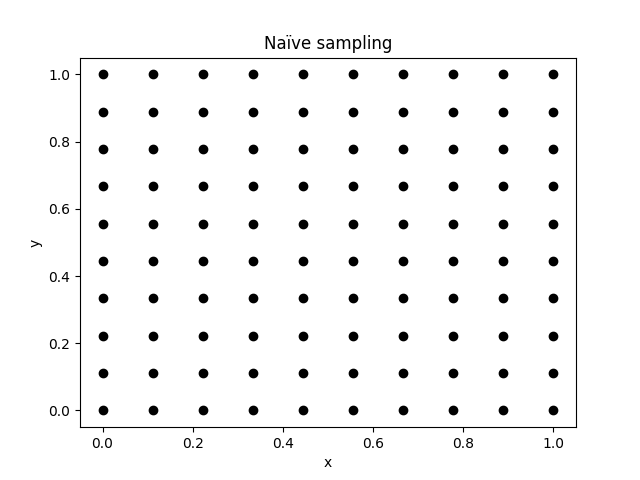
\includegraphics[width=\textwidth]{sampling-naive.png}
        \caption{Naïve strategy}
        \label{fig:sampling-naive}
    \end{subfigure}
    \hfill
    \begin{subfigure}[b]{0.49\textwidth}
        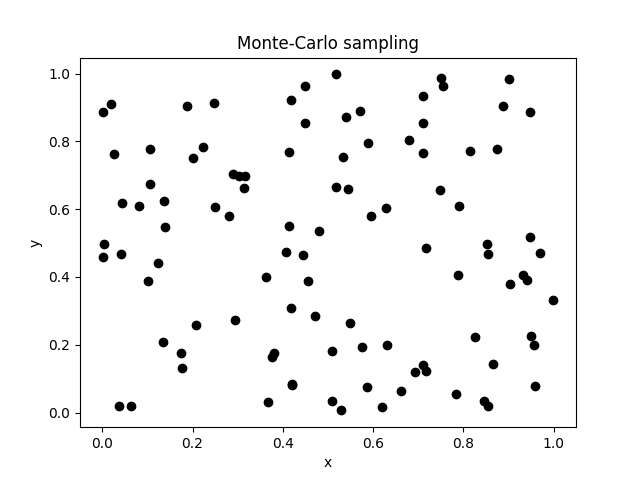
\includegraphics[width=\textwidth]{resources/images/sampling-monte-carlo.png}
        \caption{Monte-Carlo strategy}
        \label{fig:sampling-monte-carlo}
    \end{subfigure}
    \caption{Basic sampling strategies}
\end{figure}

\begin{figure}[h!]
    \centering
    \begin{subfigure}[b]{0.49\textwidth}
        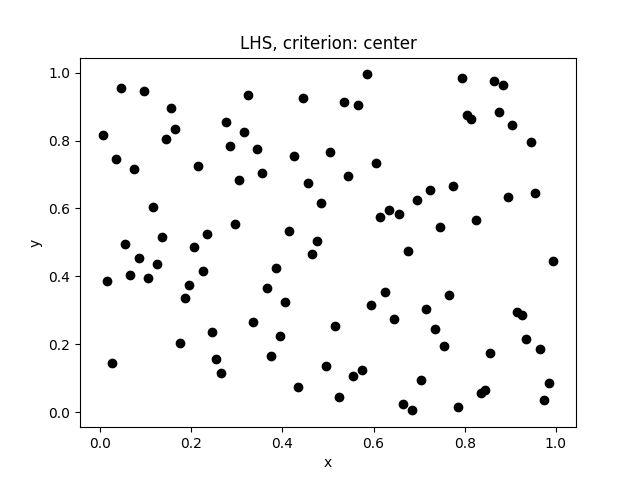
\includegraphics[width=\textwidth]{resources/images/sampling-lhs-center.png}
        \caption{LHS with center criterion}
        \label{fig:sampling-lhs-center}
    \end{subfigure} 
    \hfill
    \begin{subfigure}[b]{0.49\textwidth}
        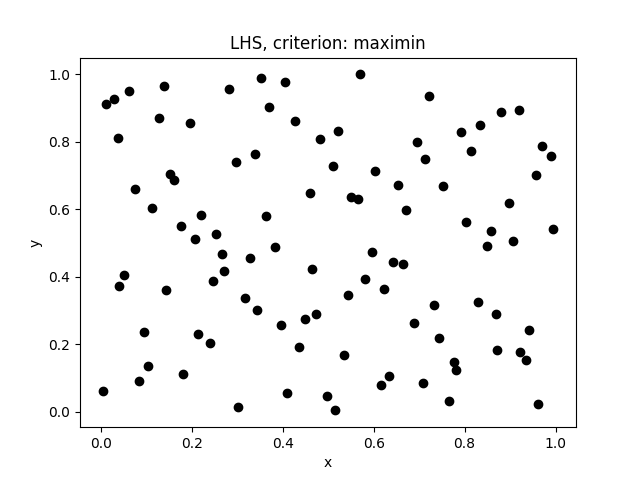
\includegraphics[width=\textwidth]{resources/images/sampling-lhs-maximin.png}
        \caption{LHS with max min distance criterion}
        \label{fig:sampling-lhs-maximin}
    \end{subfigure} 
    \hfill
    \begin{subfigure}[b]{0.49\textwidth}
        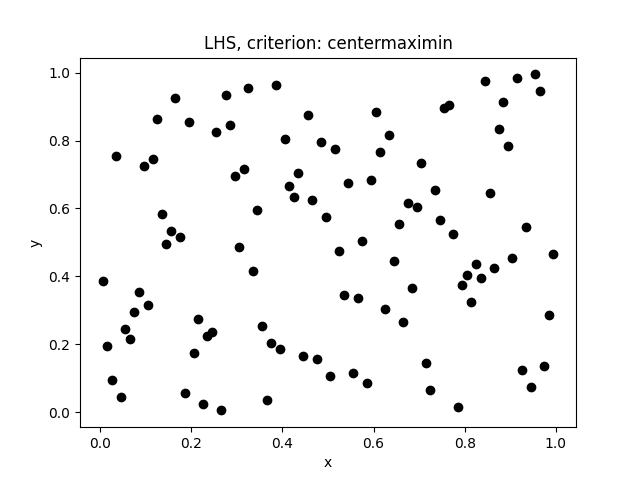
\includegraphics[width=\textwidth]{resources/images/sampling-lhs-centermaximin.png}
        \caption{LHS with max min distance and center criterion}
        \label{fig:sampling-lhs-centermaximin}
    \end{subfigure} 
    \hfill
    \begin{subfigure}[b]{0.49\textwidth}
        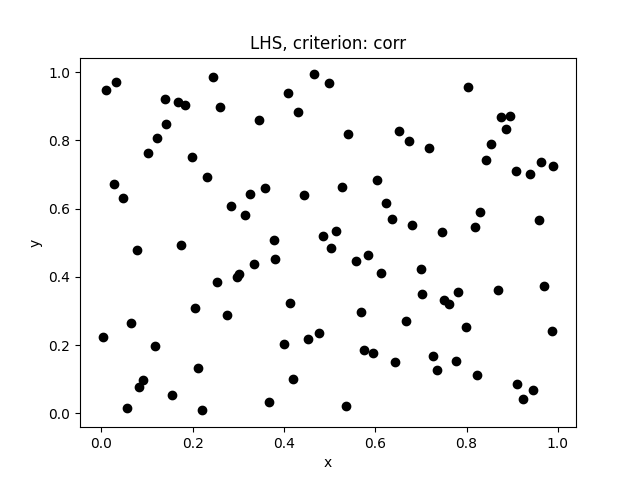
\includegraphics[width=\textwidth]{resources/images/sampling-lhs-corr.png}
        \caption{LHS with correlation criterion}
        \label{fig:sampling-lhs-corr}
    \end{subfigure} 
    \caption{Latin hypercube sampling strategies with every criterion}
\end{figure}

From these 2-dimensional illustration it is clear that the latin hypercube sampling performs best, the naive sampling featuring too much regularities that is not wanted, as they may introduce some bias, and Monte-Carlo sampling tends to make more clusters of samples, that would be inefficient (indeed, making two times the same simulation is useless).

The number of points is set quite arbitrarily to 2000. This leads to an average of $\sqrt[6]{2000} = 3.550$ points per dimension, if the points had been placed on a 6-dimensional grid in the input space. 

\subsection{Generation of the dataset}

With the input samples now obtained, the next step is now to compute the simulations on each of these points.

But this task is not trivial since the data that corresponds to these exact configuration is not available. It is thus needed to craft some new simulation settings given a reference, that is the year 2019.

\subsubsection{Adjusting functions}
To address this, Dispa-SET provides utility functions that adjust the installed capacities within the power generation fleet.

% These adjusting functions were specifically developped for this topic by Vidal in her master thesis \cite{carlas-thesis}.

\begin{itemize}
    \item \texttt{adjust\_flexibility} modifies installed capacities to reach the desired $Share_{flex}$.
    
    To do so, it first computes the target capacity, by multiplying the total capacity by the desired $Share_{flex}$. It then add or subtracts the missing or exceeding flexible unit power capacity to each zone, weighting by their total capacity. Equation \ref{equation:flex-cap-weight} gives an approximation of the update, but the full algorithm is presented in Algorithm \ref{algo:adjust_flex}.

    \begin{equation}
        PowerCap_{z,new} = PowerCap_{z,old} + \frac{PowerCap_{z,old}}{\sum_x PowerCap_{x,old}} (target-actual)
        \label{equation:flex-cap-weight}
    \end{equation}

    \begin{algorithm}[h]
        \caption{Adjust\_flexibility algorithm} \label{algo:adjust_flex}
        \begin{algorithmic}[1]
            \If {$\delta \ensuremath{>} 0$}: 
                \State $remain \gets \delta$
                \For{$z \in\ zones$}
                \State $weight \gets \frac{total_{z}}{current\_total\_cap \, - \, cum\_sum_{z}+total_{z}}$
                \State $added\_cap \gets min (weight \cdot remain, total_{z} - flex_{z}$)
                \State $new\_flex\_cap_{z} \gets flex_{z} + added\_cap$
                \State $new\_slow\_cap_{z} \gets slow_{z} - added\_cap$
                \EndFor
            \ElsIf{$\delta < 0$}: 
                \State $remain \gets - \delta$
                \For{$z \in\ zones$}
                \State $weight \gets \frac{total_{z}}{current\_total\_cap-cum\_sum_{z}+total_{z}}$
                \State $removed\_cap \gets min (weight \cdot remain, flex_{z}$)
                \State $new\_flex\_cap_{z} \gets flex_{z} - removed\_cap$
                \State $new\_slow\_cap_{z} \gets slow_{z} + removed\_cap$
                \EndFor
            \Else
            \State $new\_flex\_cap_{z} \gets flex_{z}$
            \State $new\_slow\_cap_{z} \gets slow_{z}$
            \EndIf
        \end{algorithmic}
    \end{algorithm}

    Depending on the sign of the flexibility difference $\delta$, the remainder variable is set and the algorithm loops over each zones, computes a ratio corresponding approximately to how much the considered zone has to contribute to the change. Then the amount of flexible generation capacity is added or removed accordingly.

    \item \texttt{adjust\_capacity} applies a linear scaling to the power output of some given set of units, in particular, it will be called multiples times to adjust the storage, PV and wind capacities.
    
    Scaling factors applied to match desired values are summarized in Table \ref{table:scaling-factors}.

    \begin{table}[h]
        \centering
        \begin{tabular}{|l l|}
            \hline  
            Units              & Scaling factor    \\ \hline
            $Storage_{units}$  & $Share_{storage}$ \\ 
            $Wind_{units}$     & $\frac{CapacityRatio \cdot Share_{wind}}{CF_{wton}}$ \\
            $PV_{units}$       & $\frac{CapacityRatio \cdot Share_{PV}}{CF_{PV}}$ \\ \hline
        \end{tabular}
        \caption{Scaling factors applied to different units}
        \label{table:scaling-factors}
    \end{table}

    \item \texttt{adjust\_rntc} applies a linear scaling to each zonal NTC time series.
\end{itemize}

\subsubsection{Extracted outputs}

Each simulation generates multiple outputs beyond curtailment and lost load values, some other outputs variables are extracted from the simulations, although not immediately exploited.

Of course, these may prove to be useful for future research.

All the outputs extracted from the simulations are displayed in Table \ref{table:values-extracted}.

\begin{table}[h]
    \centering
    \begin{tabular}{|l c|l c|}
		\hline
		Parameter & Unit & Parameter & Unit \\
		\hline
		Cost            & €/MWh & Shedding & TWh \\
		Congestion      & h     & LostLoad & TWh \\
		PeakLoad        & MW    & CF gas  & [$\cdot$] \\
		MaxCurtailment  & MW    & CF nuc (nuclear)  & [$\cdot$] \\
		MaxLoadShedding & MW    & CF wat (water)  & [$\cdot$] \\
		Demand          & TWh   & CF win (wind)  & [$\cdot$] \\
		NetImports      & TWh   & CF sun  & [$\cdot$] \\
		Curtailment     & TWh   &  &  \\
		\hline
	\end{tabular}
	\caption{Values extracted from each simulations}
	\label{table:values-extracted}
\end{table}

Distinction should be made between the $Shedding$ and the $LostLoad$. The former is a consequence of voluntary action, following set rules between consumers and producers. The latter is a consequence of additional variables added to Dispa-SET to reduce the infeasibility issues, assigning a high cost to the capacity the system is not able to generate due to maximum capacity and ramping constraint being reached. The Energy Not Served (ENS), is defined as the sum of $Shedding$ and $LostLoad$, and thus accounts for the actual difference between the demand and the production predicted by Dispa-SET.

\subsubsection{Dataset creation}

With the help of the adjusting functions, creating a whole dataset now comes down to generate samples from LHS as previously discussed, adjusting the reference simulation setting to each sample, run the simulation and extract the desired features from the outputs.

As this whole process is be completely automated, it is pretty easy to obtain a second dataset, based on a different LHS. In particular, a smaller dataset is interesting for the validation and testing stages of the surrogate model, as will be elaborated in subsection \ref{ssec:val-testing}.

\subsection{Implementation}

Running all of these simulation is not feasible on a basic hardware. A single MILP simulation typically takes around two hours to complete on the cluster, as the latin hypercube sampling targeted 2000 simulations, yielding to 4000 hours or 166.6 days if the simulation are run sequentially. Moreover, the testing phase also requires a significant amount of runs. This arises the need for the cluster use, and thus of submitting these as jobs on the cluster.

As the NIC5 cluster, provided by CÉCI, is obviously shared, one needs to manage the submitted jobs appropriately. In our case, we simply have the same program to be run multiple of times, that are jobs independent of each other, running the linear programming software used by Dispa-SET, GAMS (General Algrbraic Modeling Language) \cite{GAMS}.

\subsubsection{Steps}
For a complete experiment to be completed, these steps have to be followed:
\begin{enumerate}
    \item Generating the reference simulation (cfr Section \ref{section:reference-simulation}), to extract the data that will be manipulated by the adjusting function
    \item For each sample, do:
    \begin{enumerate}
        \item Call the adjusting function and create the simulation directory, with all the simulation input data
        \item Call GAMS in this simulation directory
        \item Fetch GAMS outputs in this directory
    \end{enumerate}
\end{enumerate}

\subsubsection{Scripts and code}

All the files for this section lie in the \texttt{data-generation} folder.

The steps presented above almost map to a script or function written. The flow of the dataset generation is as described here.

\begin{enumerate}
    \item The SLURM (Simple Linux Utility for Resource Management) script \texttt{main.sh} is submitted on the cluster. It fetches relevant data in the \texttt{config.py} script.
    \item It submits the generation of the reference simulation as another job on the cluster and waits for its completion.
    \item It calls \texttt{sampling.py} with argument \texttt{--sample-only}, that will create the \texttt{samples.csv} file containing all the samples.
    \item It prepares the file \texttt{dataset.csv} by writing its header line.
    \item It finally runs the bash script \texttt{launch-job-series.sh}, with serie index 0, that will submit some fixed number of sample jobs, as an array, through the SLURM script \texttt{launch-simulation-jobs.sh}.
    \item Each sample job runs:
    \begin{enumerate}
        \item The simulation directory is prepared by calling the \texttt{sampling.py} script with argument \texttt{--prepare-one} and the index of this simulation (it reads the corresponding line in \texttt{samples.csv}).
        \item GAMS is called on the simulation directory.
        \item The simulation results are read with \texttt{read\_results.py --single}, then outputted to \texttt{dataset.csv}.
        \item The simulation directory is cleaned.
    \end{enumerate}
\end{enumerate}

This list is not exhaustive, see the Annex for a complete version.

\subsubsection{Technical aspects}

During the creation of this set of scripts, some technical details require specific attention:
\begin{itemize}
    \item The GAMS solver offers options to define the number of threads to do the computations, that number of threads cannot exceed the number of allocated CPUs by SLURM for that job, as it would disturb the node on which it is running, including affecting unrelated jobs.
    
    The thread setting in the \texttt{UCM\_h.gms} file generated by Dispa-SET is set to 16 by default, this line may be removed if one wants to set it manually through the command line, as the file input takes precedence over the command-line value set.
    \item The total amount of each prepared simulation directory is too large to fit on the allocated disk memory on the \texttt{\$HOME} partition on the cluster. Moreover, for efficiency it is better to use the \texttt{\$GLOBALSCRATCH} file system.
    \item The Dispa-SET ajdusting function do not write adjusted data to a directory if this directory already exists before the function is called. That is, the directory containing the simulation files should not be created beforehand.
    \item Due to SLURM limiting the maximum number of jobs a user can have in the submit queue, queuing all the simulation jobs at once is not possible. Moreover, the number of simulation appeared to cause issues with the SLURM maximum array size.

    This is the reason why \texttt{launch-job-series.sh} exists. The script takes as an argument the serie index $i$, then starts a [$0:399$] array of \texttt{launch-simulation-jobs.sh} jobs, with $i$ as an argument. As the latter script has also access to its array index via SLURM environment variables, it can compute the intended simulation index, that covers the [$400i:400i+399$] range. The next series is queued with the job array as a dependency, so that it is not launched before the current series terminated.
\end{itemize}

\subsubsection{Unsuccessful simulations}

During the execution of the simulation, it appeared that for some of them GAMS was completely stuck at some point, hence wasting resources and preventing the other simulations to start by keeping available CPUs busy.

A timeout on the GAMS simulation has therefore been set, after looking at the typical duration of a "regular" simulation. The simulation that were timed out had thus the corresponding error message in their output, that can be checked when reading the results.

Hence, we can label the samples whose simulation failed with an additional error field in the dataset, and compare them to the other. Typically, around 10\% of the simulation fail, in this case 218 over 2400 total.

Loading this dataset and separating the successful simulations from failing ones, and extracting meaningful metrics from both, it appeared that the failing simulations featured an average share flexibility significantly higher than the other, while the other input parameters seemed around the same. The share of flexible generation is taken in the $[0.01, 0.99]$ interval, and the average of failing simulations is around $0.49$ higher than the average of the successful ones.

To further validate our observation, the quantiles of the distribution of the share of flexible generation in the stalling settings are explored, and it appears that they lie really high, the first one (25\%) is around 0.9, the median lies near 0.95 and the third one (75\%) is around 0.96. 

More decisively, the maximum value of a successful simulation is 0.9011, while the minimum value of a stalling simulation is 0.9015, that is, slightly more than the max of valid simulations. Thus, there exists a net boundary between the simulation that run successfully and the other. 

The distribution of $ShareFlex$ values in both part of the dataset is depicted as boxplots in Figure \ref{fig:stalling-simulations}

\begin{figure}[h]
    \centering
    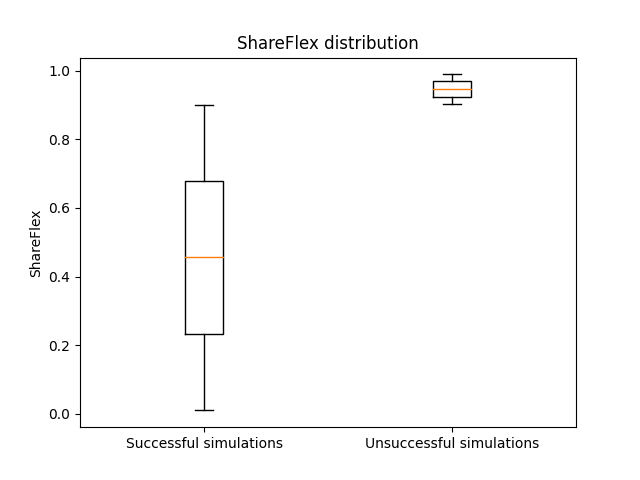
\includegraphics[width=0.6\textwidth]{resources/images/share-flex-boxplots.png}
    \caption{Distributions of the $ShareFlex$ parameter value in the unsuccessful simulations against successful simulation. The distributions of the other parameters are similar.}
    \label{fig:stalling-simulations}
\end{figure}

As a consequence, the validity region for the surrogate model has to be updated, as there is no way of producing an estimate of the outputs on a region where no sample was simulated correctly.

This issue is interpreted as the simulations with too high flexibility are harder to solve than the other, as the system has a lot of options to choose from when confronted to a change in demand, yeilding an exponential growth of the realistic evolutions of the system.

It is noteworthy that in about 30\% of the simulation, a division by zero error was also stated. Since this happens in the preprocessing, it has no influence on the results and this error is discarded.

% It would also be useful to find in which equation this happens for debugging purposes.

\subsubsection{Dataset fields}

For completeness, all the fields in the created dataset in \texttt{dataset.csv} are shown in Table \ref{table:dataset-fields}.

Only two of these, $LoadShedding$ and $Curtailment$ are actually used to train the surrogate model, and six as the model features. As the marginal cost of including all the other outputs is null, they are saved as well in case someone would find a use for it in the future.

\begin{table}[h]
    \centering
	\begin{tabular}{|l c|l c|}
		\hline
		Parameter & Unit & Parameter & Unit \\
		\hline
		Cost             & €/MWh & Curtailment          & \% \\
		Congestion       & h     & MaxLoadSheddingShare\tablefootnote{The MaxLoadSheddingShare is taken as a fraction of the demand at the time.} & \% \\
		PeakLoad         & MW    & CF gas         & [$\cdot$] \\
		MaxCurtailment   & MW    & CF nuc         & [$\cdot$] \\
		MaxLoadShedding  & MW    & CF wat         & [$\cdot$] \\
		Demand           & TWh   & CF win         & [$\cdot$] \\
		NetImports       & TWh   & CF sun         & [$\cdot$] \\
		{\color{blue} Curtailment}      & \%   & {\color{green} Capacity ratio} & [$\cdot$] \\
		{\color{blue} Shedding}         & \%   & {\color{green} Share flex}     & [$\cdot$] \\
		LostLoad         & TWh   & {\color{green} Share sto}   & [$\cdot$] \\
        MaxRESGeneration & MW    & {\color{green} Share Wind}  & [$\cdot$] \\
        TotalGeneration  & TWh   & {\color{green} Share PV}    & [$\cdot$] \\
        ShareRESGeneration & \%  & {\color{green} rNTC}        & [$\cdot$] \\
        LoadShedding & [$\cdot$] & & \\
		\hline
	\end{tabular}
	\caption{Dataset fields. "\%" as a unit means a unitless ratio multiplied by 100. Elements displayed in green correspond to the six features, and elements in blue the two target outputs.}
	\label{table:dataset-fields} 
\end{table}